\begin{figure}[t]
\centering
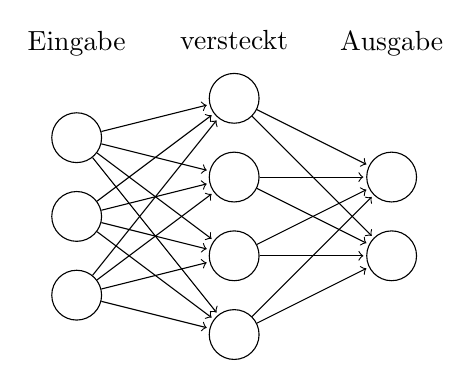
\begin{tikzpicture}
  \tikzstyle{node}=[circle,draw, minimum width=18pt, inner sep=0pt, fill=white]
  \tikzstyle{edge}=[->, shorten >= 1pt]

  \node[rectangle, inner sep=0pt] at (-2, 2.2) {Eingabe};
  \node[rectangle, inner sep=1pt] at (0,  2.24) {versteckt};
  \node[rectangle, inner sep=0pt] at (2,  2.2) {Ausgabe};

  \node[node] (a1) at (-2, -1) {};
  \node[node] (a2) at (-2, 0)  {};
  \node[node] (a3) at (-2, 1)  {};

  \node[node] (b1) at (0, -1.5) {};
  \node[node] (b2) at (0, -0.5) {};
  \node[node] (b3) at (0, 0.5)  {};
  \node[node] (b4) at (0, 1.5)  {};

  \node[node] (c1) at (2, -0.5) {};
  \node[node] (c2) at (2, 0.5)  {};

  \path[edge] (a1) edge (b1);
  \path[edge] (a1) edge (b2);
  \path[edge] (a1) edge (b3);
  \path[edge] (a1) edge (b4);
  \path[edge] (a2) edge (b1);
  \path[edge] (a2) edge (b2);
  \path[edge] (a2) edge (b3);
  \path[edge] (a2) edge (b4);
  \path[edge] (a3) edge (b1);
  \path[edge] (a3) edge (b2);
  \path[edge] (a3) edge (b3);
  \path[edge] (a3) edge (b4);
  \path[edge] (b1) edge (c1);
  \path[edge] (b1) edge (c2);
  \path[edge] (b2) edge (c1);
  \path[edge] (b2) edge (c2);
  \path[edge] (b3) edge (c1);
  \path[edge] (b3) edge (c2);
  \path[edge] (b4) edge (c1);
  \path[edge] (b4) edge (c2);
\end{tikzpicture}
\caption[Feedforward-Netz]{Beispiel eines Feedforward-Netzes mit drei vollverbundenen Schichten von einer Eingabe mit drei Neuronen zu einer Ausgabe mit zwei Neuronen und einer dazwischenliegenden versteckten Schicht.}
\label{fig:feedforward}
\end{figure}
